\documentclass[tikz,border=0cm]{standalone}
\usepackage[a0paper,margin=1in]{geometry}
\usetikzlibrary{calc}
\usetikzlibrary{decorations.pathmorphing,fit}
\usepackage{qrcode}

\usepackage[giveninits=true,isbn=false,doi=true,
url=false,sorting=none,style=nature,backend=biber,
maxbibnames=9,maxcitenames=1,mincitenames=1,
citestyle=verbose-ibid]{biblatex}
\addbibresource{pezzuto.bib}

% colors
\definecolor{ccmcyellow}{RGB}{254,196,54}
\definecolor{ccmcblue}{RGB}{8,65,96}
\definecolor{ccmcred}{rgb}{0.7,0.2,0.2}
\definecolor{icsyellow}{RGB}{254,223,101}

% fonts
%\usepackage{type1cm}
%\usepackage{cmbright}
\usepackage{fetamont}
\usepackage{fp}
\edef\myfontscale{1.1}
%% scalable vector fonts
\edef\fontSizeX{12}\edef\fontSizeY{14}
\FPupn{\resulttinyX}{myfontscale fontSizeX * 2 round}
\FPupn{\resulttinyY}{myfontscale fontSizeY * 2 round}
\renewcommand*{\tiny}{\fontsize{\resulttinyX}{\resulttinyY}\selectfont}

\edef\fontSizeX{14.4}\edef\fontSizeY{18}   
\FPupn{\resultscriptsizeX}{myfontscale fontSizeX * 2 round}
\FPupn{\resultscriptsizeY}{myfontscale fontSizeY * 2 round}
\renewcommand*{\scriptsize}{\fontsize{\resultscriptsizeX}{\resultscriptsizeY}\selectfont}

\edef\fontSizeX{17.28}\edef\fontSizeY{22}
\FPupn{\resultfootnotesizeX}{myfontscale fontSizeX * 2 round}
\FPupn{\resultfootnotesizeY}{myfontscale fontSizeY * 2 round}
\renewcommand*{\footnotesize}{\fontsize{\resultfootnotesizeX}{\resultfootnotesizeY}\selectfont}

\edef\fontSizeX{20.74}\edef\fontSizeY{25}
\FPupn{\resultsmallX}{myfontscale fontSizeX * 2 round}
\FPupn{\resultsmallY}{myfontscale fontSizeY * 2 round}
\renewcommand*{\small}{\fontsize{\resultsmallX}{\resultsmallY}\selectfont}

\edef\fontSizeX{24.88}\edef\fontSizeY{30}
\FPupn{\resultnormalsizeX}{myfontscale fontSizeX * 2 round}
\FPupn{\resultnormalsizeY}{myfontscale fontSizeY * 2 round}
\renewcommand*{\normalsize}{\fontsize{\resultnormalsizeX}{\resultnormalsizeY}\selectfont}

\edef\fontSizeX{29.86}\edef\fontSizeY{37}
\FPupn{\resultlargeX}{myfontscale fontSizeX * 2 round}
\FPupn{\resultlargeY}{myfontscale fontSizeY * 2 round}
\renewcommand*{\large}{\fontsize{\resultlargeX}{\resultlargeY}\selectfont}

\edef\fontSizeX{35.83}\edef\fontSizeY{45}
\FPupn{\resultLargeX}{myfontscale fontSizeX * 2 round}
\FPupn{\resultLargeY}{myfontscale fontSizeY * 2 round}
\renewcommand*{\Large}{\fontsize{\resultLargeX}{\resultLargeY}\selectfont}

\edef\fontSizeX{43}\edef\fontSizeY{54}
\FPupn{\resultLARGEX}{myfontscale fontSizeX * 2 round}
\FPupn{\resultLARGEY}{myfontscale fontSizeY * 2 round}
\renewcommand*{\LARGE}{\fontsize{\resultLARGEX}{\resultLARGEY}\selectfont}

\edef\fontSizeX{51.6}\edef\fontSizeY{64}
\FPupn{\resulthugeX}{myfontscale fontSizeX * 2 round}
\FPupn{\resulthugeY}{myfontscale fontSizeY * 2 round}
\renewcommand*{\huge}{\fontsize{\resulthugeX}{\resulthugeY}\selectfont}

\edef\fontSizeX{61.92}\edef\fontSizeY{77}
\FPupn{\resultHugeX}{myfontscale fontSizeX * 2 round}
\FPupn{\resultHugeY}{myfontscale fontSizeY * 2 round}
\renewcommand*{\Huge}{\fontsize{\resultHugeX}{\resultHugeY}\selectfont}

\edef\fontSizeX{74.3}\edef\fontSizeY{93}
\FPupn{\resultveryHugeX}{myfontscale fontSizeX * 2 round}
\FPupn{\resultveryHugeY}{myfontscale fontSizeY * 2 round}
\newcommand*{\veryHuge}{\fontsize{\resultveryHugeX}{\resultveryHugeY}\selectfont}

\edef\fontSizeX{89.16}\edef\fontSizeY{112}
\FPupn{\resultVeryHugeX}{myfontscale fontSizeX * 2 round}
\FPupn{\resultVeryHugeY}{myfontscale fontSizeY * 2 round}
\newcommand*{\VeryHuge}{\fontsize{\resultVeryHugeX}{\resultVeryHugeY}\selectfont}

\edef\fontSizeX{107}\edef\fontSizeY{134}
\FPupn{\resultVERYHugeX}{myfontscale fontSizeX * 2 round}
\FPupn{\resultVERYHugeY}{myfontscale fontSizeY * 2 round}
\newcommand*{\VERYHuge}{\fontsize{\resultVERYHugeX}{\resultVERYHugeY}\selectfont}

% set the normalfont (default)
\renewcommand*{\normalfont}{\normalsize}

\usepackage[none]{hyphenat}

\usepackage[sfmath]{kpfonts}
\renewcommand*\familydefault{\sfdefault}
\usepackage[T1]{fontenc}

\usepackage{amsmath,amssymb,bm}
\usepackage{wrapfig}
\usepackage{microtype}
\usepackage{booktabs}

\newcommand{\KK}{\mathbf{K}}
\newcommand{\MM}{\mathbf{M}}
\newcommand{\AAmat}{\mathbf{A}}
\newcommand{\tD}{\mathbf{D}}
\newcommand{\WW}{\mathcal{W}}
\DeclareMathOperator{\GammaFun}{\Gamma}
\DeclareMathOperator{\Cov}{Cov}
\usepackage{mathtools}
\DeclarePairedDelimiter{\floor}{\lfloor}{\rfloor}

%\newcommand\ipanel[2]{\valign{##\vfill\cr
%    \rlap{#2}\cr
%    \rlap{\bfseries#1}\cr
%    \phantom{#2}\cr
%}}

\begin{document}
\begin{tikzpicture}[x=841mm,y=1189mm]
\draw[blue!10!white,use as bounding box] (0,0) rectangle (1,1);

%%%% title %%%%
\begingroup
\pgfmathsetseed{3672}
\node[anchor=north west,fill=icsyellow,
text width=117cm,inner sep=2cm,decorate,
decoration={random steps,segment length=1cm,amplitude=4mm},
draw=ccmcyellow,line width=2mm]
(title)
at ($(current bounding box.north west)+(-1cm,1cm)$)
{
{\ffmfamily\Huge\bfseries
Learning cardiac activation maps from 12-lead ECG\\[0.5em]
with multi-fidelity Bayesian optimization on manifolds}

\bigskip
\newcommand{\myaff}[1]{${}^{\mathrm{(#1)}}$}
\newcommand{\affSP}{\myaff{1}}
\newcommand{\affPP}{\myaff{2}}
\newcommand{\affFSC}{\myaff{3}}
{\bfseries
Simone Pezzuto,\affSP\
Paris Perdikaris,\affPP\
Francisco Sahli Costabal.\affFSC}

\raisebox{-2mm}{
\includegraphics[height=1em]{email}}
\texttt{\footnotesize simone.pezzuto@usi.ch}

\bigskip
(1) Center for Computational Medicine in Cardiology,
    Euler Institute,
    Universit\`a della Svizzera italiana.\\
(2) Department of Mechanical Engineering and Applied Mechanics,
    University of Pennsylvania.\\
(3) Department of Mechanical and Metallurgical Engineering,
    School of Engineering,
    Pontificia Universidad Cat\'olica de Chile.\\
};
\endgroup

%%%%%%%%%%%%%%%%%%%%%%
%%%% introduction %%%%
%%%%%%%%%%%%%%%%%%%%%%

\tikzset{
  motif col/.style={inner sep=1cm,text width=24cm},
  motif title/.style={font=\bfseries\ffmfamily\Large},
}

\node[anchor=south west,motif title]
(motif title) at ($(title.south west)+(3cm,-3cm)$)
{Motivations};
\draw[line width=1mm] ($(motif title.south east)+(0,1mm)$)--++(-20cm,0);

\node[motif col,anchor=north west] (motif1) at (motif title.south west)
{
Ectopic activity in the heart can trigger deadly arrhythmias. The localization of the ectopic foci or earliest activation sites (EASs) is therefore a critical information for cardiologists in deciding the optimal treatment.
};

\node[motif col,anchor=north west] (motif2) at (motif1.north east)
{
Precision cardiology aims at creating a digital twin of the patient's heart.
Here, we focus on the problem of identifying an ectopic activation in the heart non-invasively, only by using the 12-lead ECG and imaging data.
};

\node[motif col,anchor=north west] (motif3) at (motif2.north east)
{
In this work, we formulate the identification problem as a global optimization problem, by minimizing the mismatch between the ECG predicted by a cardiac model, when paced at a given EAS, and the observed ECG during the ectopic activity. 
};

\node[fit={(motif1)(motif2)(motif3)},inner sep=0pt] (motif) {};


%%%%%%%%%%%%%%%%%
%%%% methods %%%%
%%%%%%%%%%%%%%%%%

\tikzset{
  hbox title/.style={draw=black,minimum width=39cm,text=white,
                     fill=ccmcblue,rounded corners,font=\bfseries\ffmfamily},
  hbox main/.style={fill=ccmcblue!20!white,draw,rounded corners,fill opacity=0.9,
                    text opacity=1,inner sep=5mm,text width=38cm,minimum height=43cm},
  method title/.style={font=\bfseries\ffmfamily\Large},
}

\node[anchor=north west,method title] (methods title) at ($(motif.south west)+(0,-1cm)$)
{Methods};
\draw[line width=1mm] ($(methods title.south east)+(0,1mm)$)--++(-20cm,0);

%%% Model %%%

\node[anchor=north west,hbox title]
(geoKL title) at ($(methods title.south west)+(0,-5mm)$)
{ECG in-silico model};

\node[anchor=north west,hbox main]
(geoKL1) at ($(geoKL title.south west)+(0,-5mm)$)
{
\begin{center}
\includegraphics[width=0.95\textwidth]{img/intro_models}
\end{center}

\vspace{-5mm}\begin{itemize}
\renewcommand{\labelitemi}{$\blacktriangleright$}
\renewcommand{\itemsep}{1ex}

\item \textbf{Ectopic focus}

We model the ectopic focus as a single point on the endocardium.

\item \textbf{Conduction velocity}

We consider anisotropic conduction: that is, propagation velocity
is faster in the fiber direction.

Moreover, we model a fast endocardial layer mimicking the Purkinje
network.

\item \textbf{Activation map}

We solve the anisotropic eikonal equation to extrapolate the activation
map in the tissue, given an ectopic focus and the conduction velocity.

The computer model is fast: takes only 0.4\,s to compute the map
in the biventricular model, at 1\,mm resolution.

\item \textbf{ECG simulation}

\begin{minipage}{0.7\textwidth}
With activation at hands, we construct a transmembrane potential in
the whole heart, just by shifting an action potential at the right
timing.

The ECG is simulated by solving the bidomain model in the torso.
given the transmembrane potential. The computation is feasible
thanks to the lead field approach.
\end{minipage}\hspace{2cm}
\begin{minipage}{0.2\textwidth}
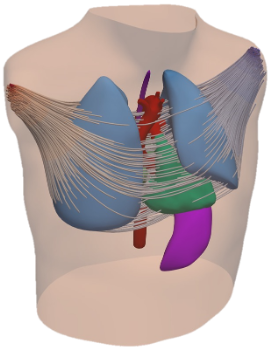
\includegraphics[width=0.8\textwidth]{img/torso}
\end{minipage}


\item \textbf{ECG mismatch}

The obtained ECG can be compared to a given patient ECG
during an extrasystole.

Therefore, we can quickly estimate the how far we are from
the true source of the extrasystole by testing multiple points.

\end{itemize}
};


%%% Optimization %%%

\node[anchor=north west,hbox title,fill=ccmcred]
(SPDE title) at ($(methods title.south west)+(41cm,-5mm)$)
{Multi-fidelity Bayesian Optimization};

\node[anchor=north west,hbox main,fill=ccmcred!20!white]
(SPDE1) at ($(SPDE title.south west)+(0,-5mm)$)
{
\vspace{-5mm}\begin{itemize}
\renewcommand{\labelitemi}{$\blacktriangleright$}
%\renewcommand{\itemsep}{1ex}

\item \textbf{Gaussian Process Regression on Surfaces}

Each point on the endocardium corresponds to number
indicating how close we are to the real ectopic site.
We extrapolate the indicator over the whole surface
with with Gaussian Process Regression (GPR).
In other words, the indicator is a linear combination
of basis functions (eigenfunctions) of the Laplace-Beltrami
operator.

\begin{center}
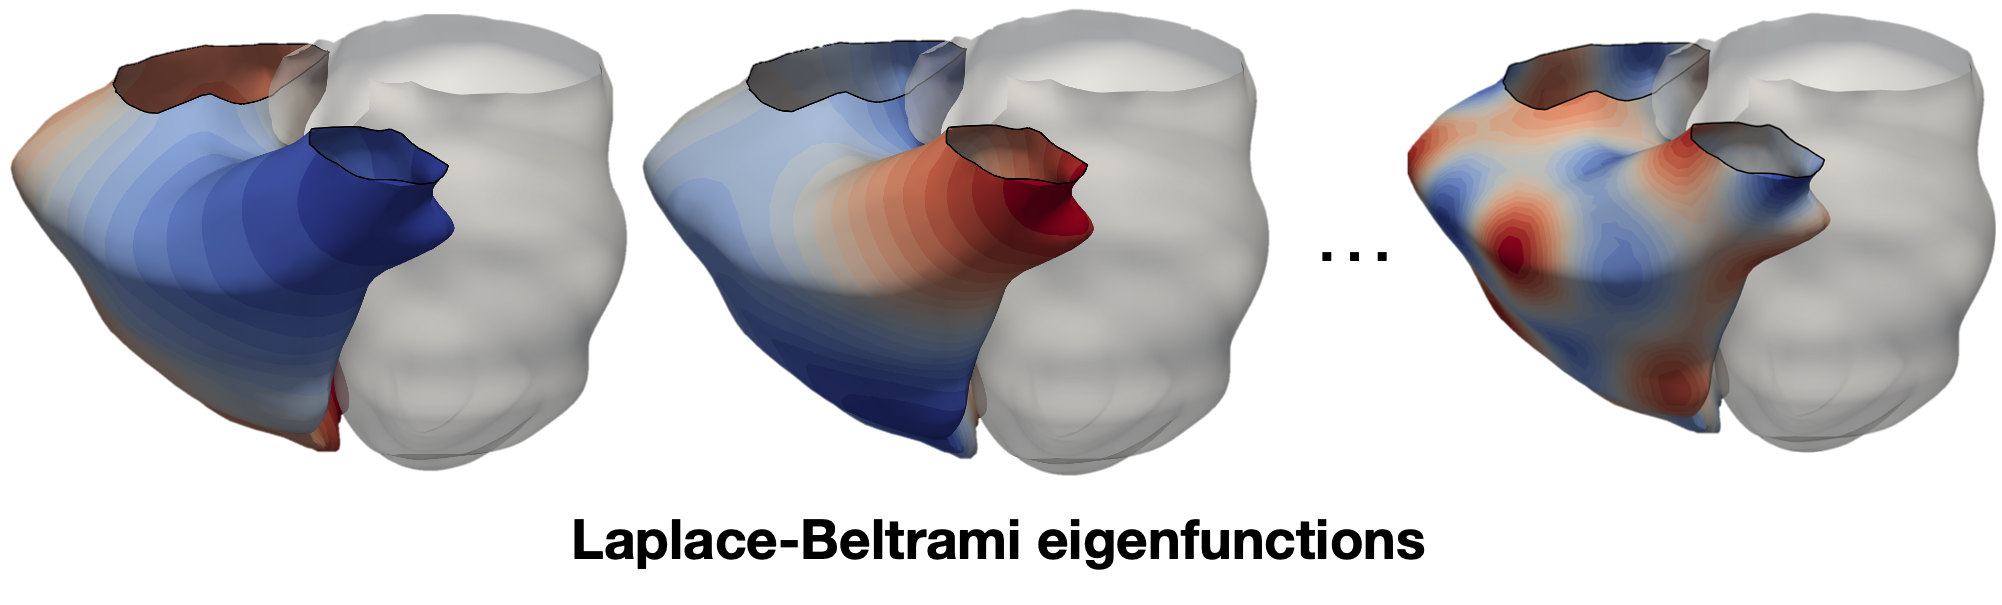
\includegraphics[width=0.95\textwidth]{img/gps}
\end{center}

\item \textbf{Bayesian Optimization}

We use active learning to probe the next candidate location.
The acquisition function is a trade-off between maximizing
the correlation with the surface ECG, and explore regions
far from already sampled points.

\item \textbf{Multi-fidelity learning}

\begin{minipage}{0.35\textwidth}
The high fidelity model is computationally expensive to query.
We use a multi-fidelity representation of the indicator, where
the correlation with to low fidelity model is exploited so
to reduce the computational burden.
Many more low fidelity points are acquired than high fidelity
points, with a comparable accuracy to the single fidelity approach,
but at a fraction of the cost.
\end{minipage}%
\begin{minipage}{0.6\textwidth}
\begin{center}
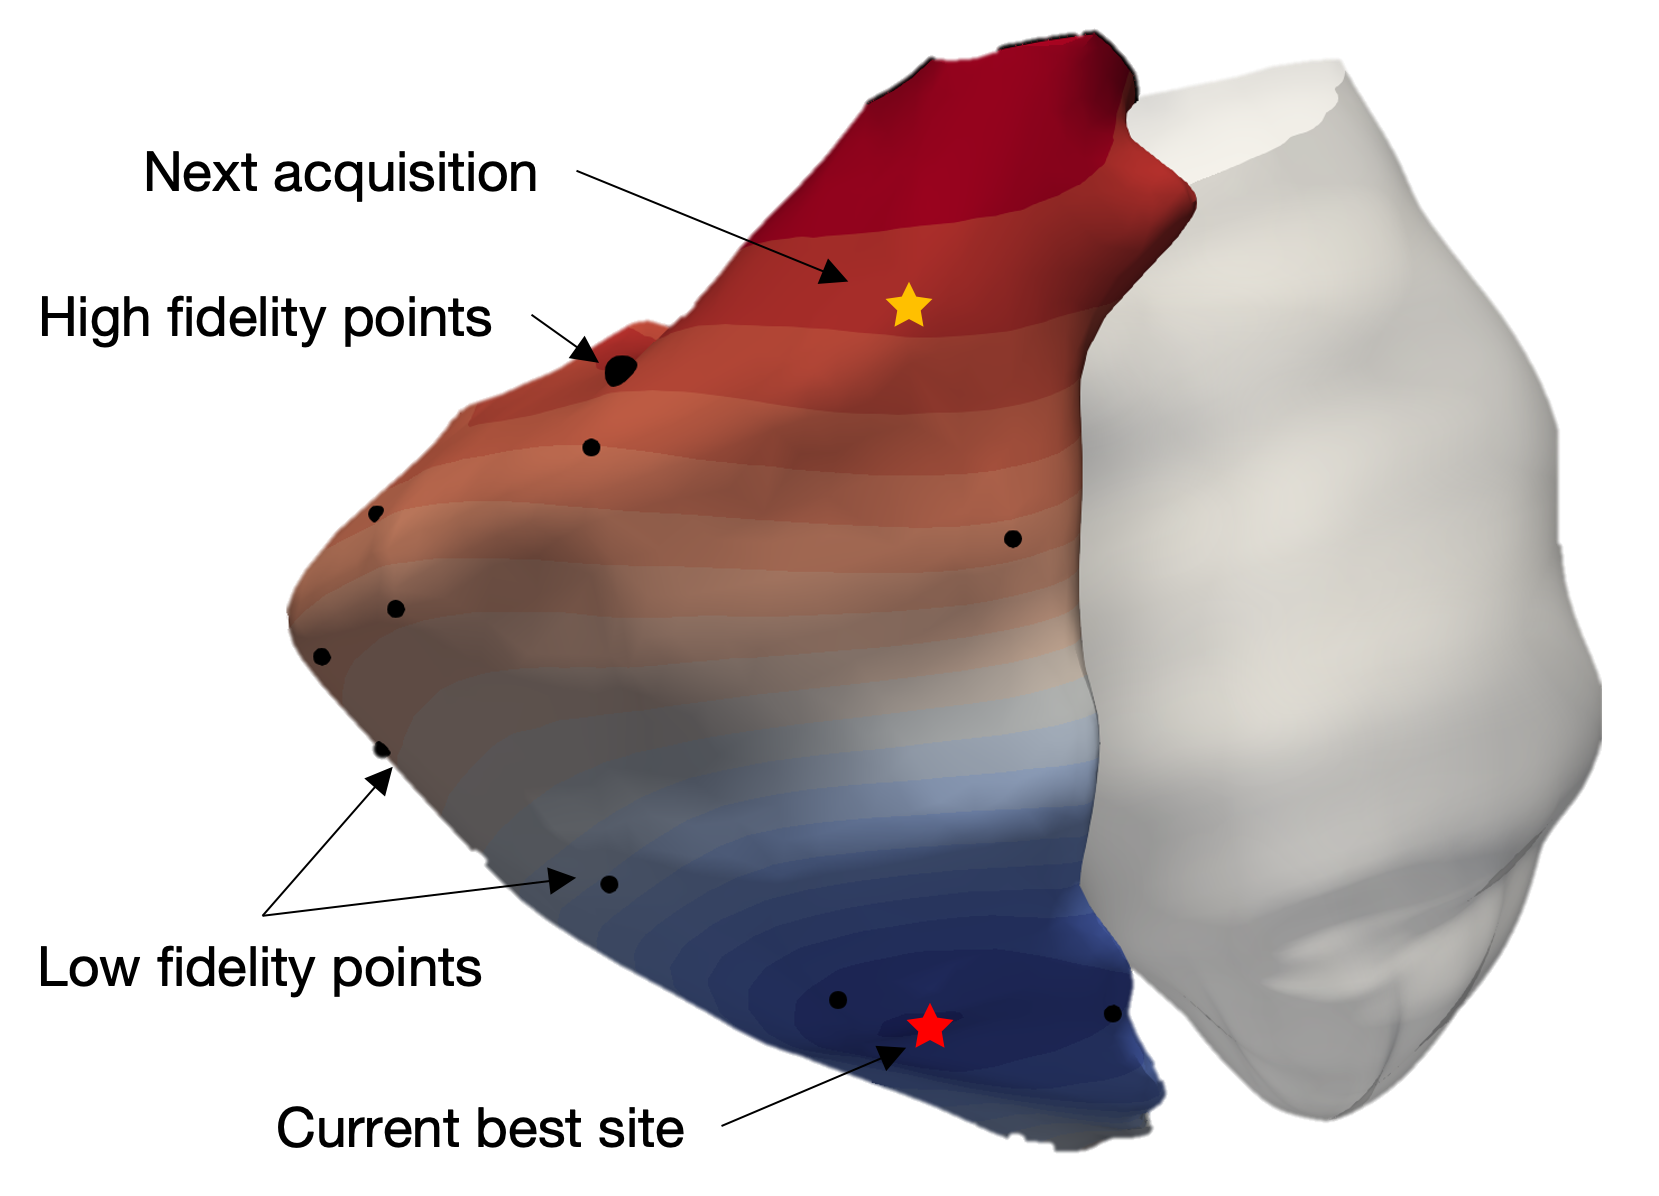
\includegraphics[width=\textwidth]{img/bayes}
\end{center}
\end{minipage}%

\end{itemize}

};

\node[fit={(geoKL title)(geoKL1)(SPDE title)(SPDE1)},inner sep=0pt] (methods) {};


%%%%%%%%%%%%%%%
%%% results %%%
%%%%%%%%%%%%%%%

\node[anchor=north west,font=\bfseries\ffmfamily\Large]
(results title) at ($(methods.south west)+(0,-3cm)$)
{Results};
\draw[line width=1mm] ($(results title.south east)+(0,1mm)$)--++(-20cm,0);

%%% ECG correlation %%%

\tikzset{
  caption text/.style={font=\footnotesize},
}

\node[anchor=north west,draw,color=white,fill=black]
(examples title) at ($(results title.south west)+(3mm,-5mm)$)
{ECG correlation};

\node[anchor=north west] (ex1) at (examples title.south west)
{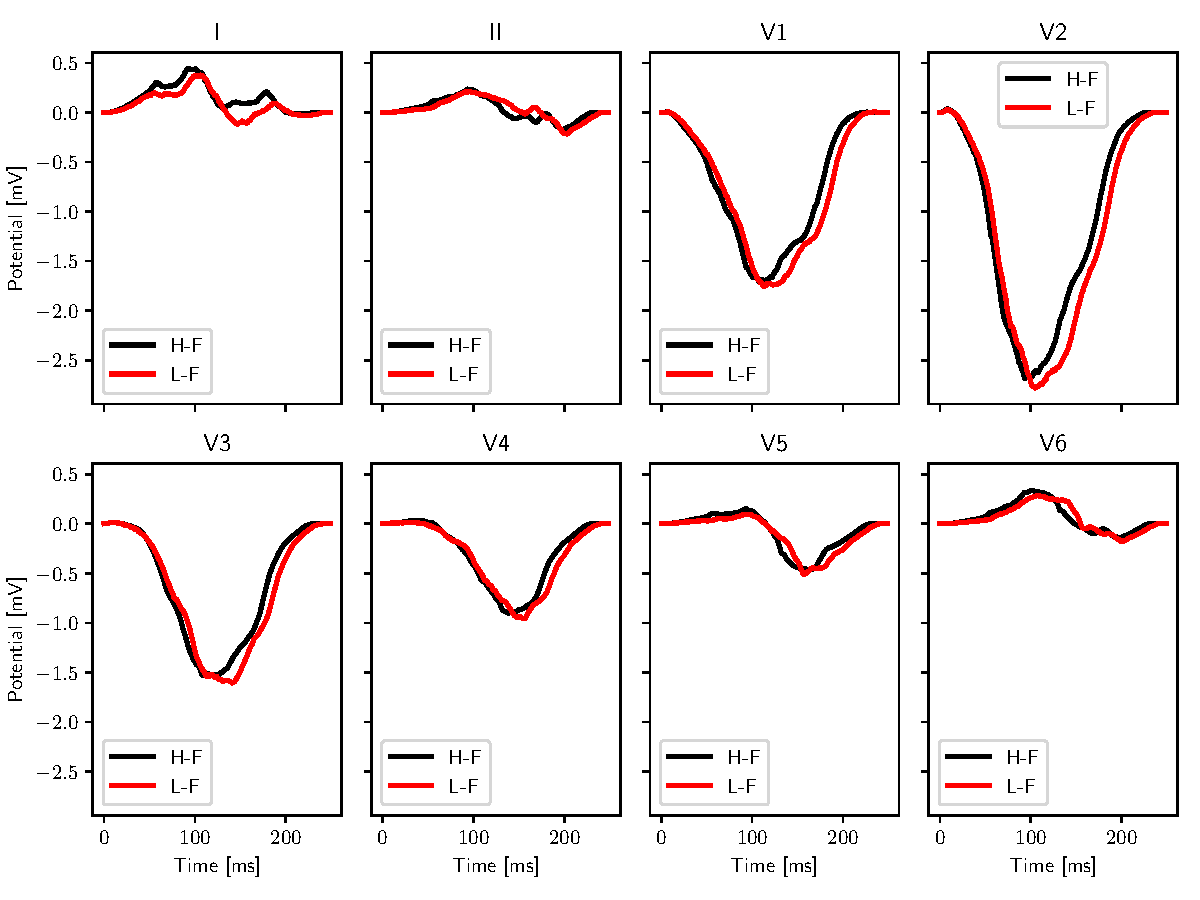
\includegraphics[width=28cm]{img/ECG_HF_vs_LF}};

\node[fit={(examples title)(ex1)},draw,inner sep=0pt] (examples) {};


%%% single fidelity %%%

\tikzset{
  img/.style={inner sep=5mm,anchor=north west},
  img label/.style={inner sep=2pt,anchor=north west,
  fill=white,opacity=0.4,text opacity=1.0,font=\bfseries},
}

\node[anchor=north west,draw,color=white,fill=black]
(comp title) at ($(examples.north east)+(5mm,0mm)$)
{Single fidelity};

\node[img] (compimg) at (comp title.south west)
{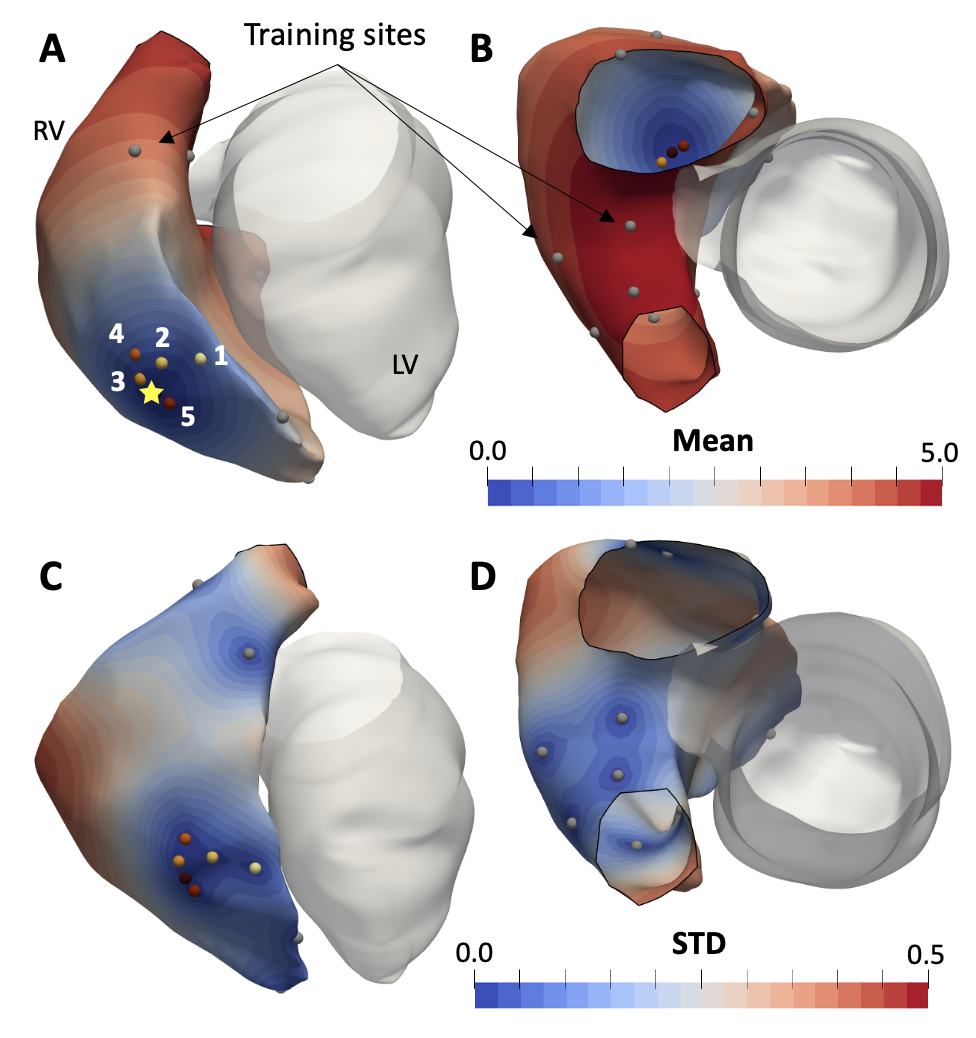
\includegraphics[width=23cm]{img/SingleFidelity_v2}};

%node[img] (comp1b) at ($(comp1a.north east)+(1cm,0)$)
%{\includegraphics[width=9.8cm]{img/stddev_SPDE}}
%node[img label] at ($(comp1b.north west)+(5mm,-5mm)$) {B}
%
%node[img] (comp1c) at ($(comp1b.north east)+(1cm,0)$)
%{\includegraphics[width=9.8cm]{img/cov_along_geodesic}}
%node[img label] at ($(comp1c.north west)+(5mm,-5mm)$) {C}
%
%node[anchor=north west,text width=34cm,caption text] (comp2) at (comp1a.south west)
%{
%$N=10\,000$ samples defined on a hollow square domain,
%uniform mesh $h=1/100$,
%squared-exponential kernel $h(d)=e^{-d^2/\rho^2}$ in geoKL
%with $\rho=0.2$ and $K=5$, $\kappa=2\sqrt{\nu}/\rho$ in SPDE.
%}
%
%node[anchor=north west,text width=17cm,caption text] (comp3) at (comp2.south west)
%{
%\textbf{GeoKL}: error in variance uniform
%with some oscillations due to approximate geodesic distance (Figure A).
%
%Cost: 26\,s setup, negligible per sample.}
%
%node[anchor=north west,text width=17cm,caption text] (comp4) at (comp3.north east)
%{
%\textbf{SPDE}:
%strong boundary effect in the variance, being significantly larger close
%to the boundary (Figure B).
%
%Cost: no setup, 3\,s per sample.
%};

\node[fit={(comp title)(compimg)},minimum height=27cm,draw,inner sep=0pt] (comp) {};


\node[anchor=north west,draw,color=white,fill=black]
(mf title) at ($(comp.north east)+(5mm,0mm)$)
{Multi fidelity};

\node[img] (mf img1) at (mf title.south west)
{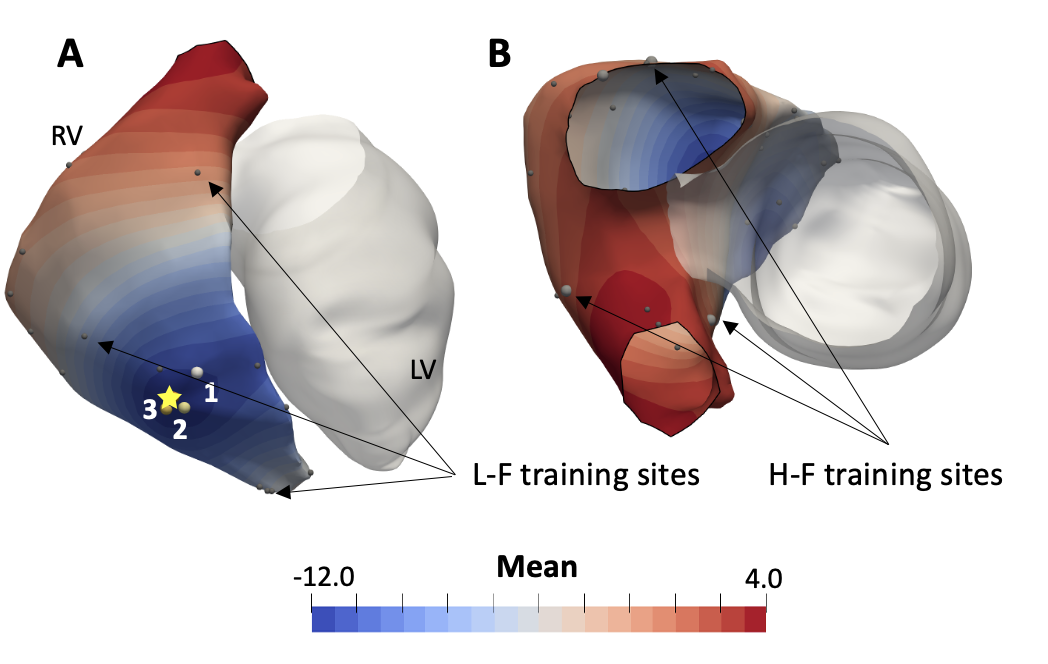
\includegraphics[width=23cm,clip,trim=0 70 0 0]{img/MultiFidelity}};

\node[img] (mf img2) at (mf img1.south west)
{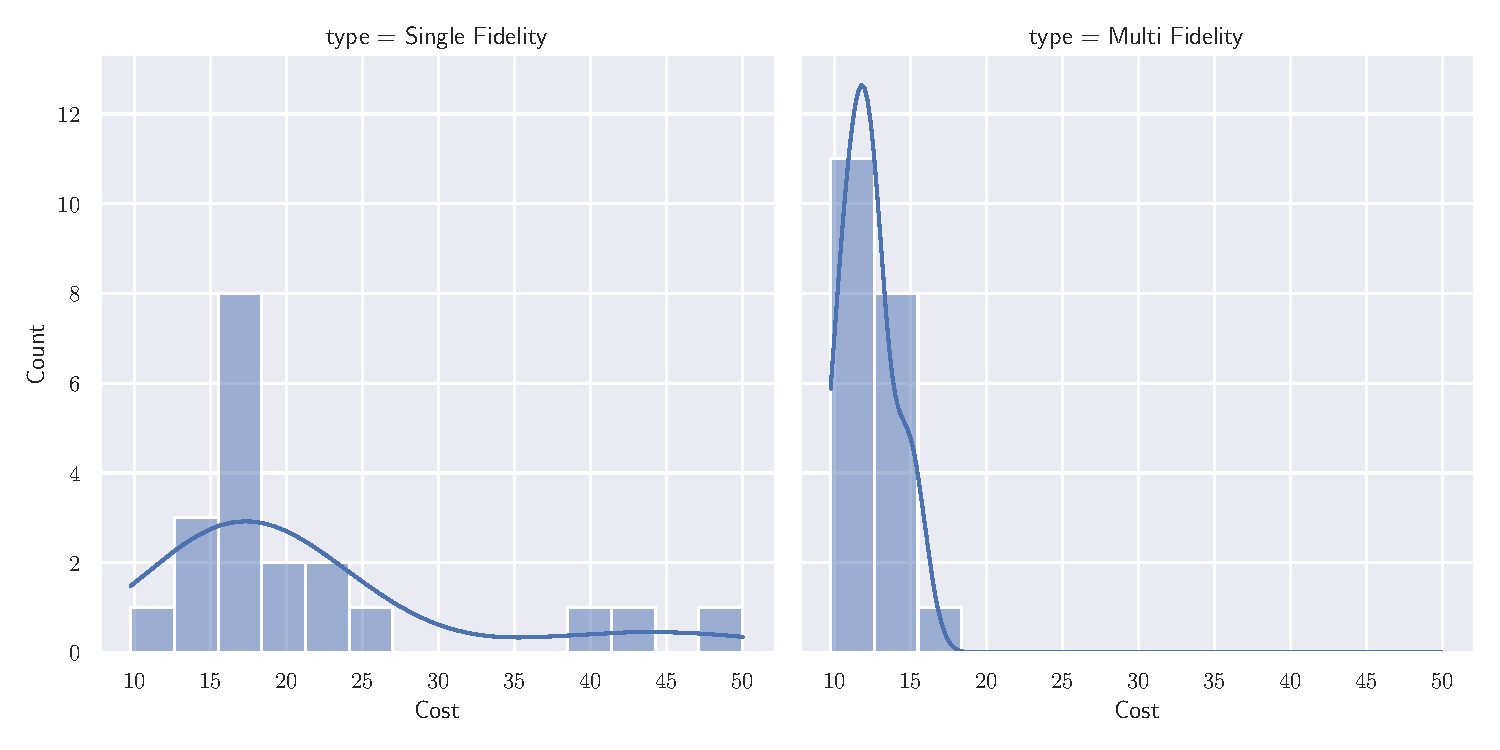
\includegraphics[width=24cm]{img/Convergence}};

\node[fit={(mf title)(mf img1)(mf img2)},minimum height=27cm,draw,inner sep=0pt] (mf) {};


\node[fit={(examples)(comp)},inner sep=0pt] (resbox) {};

%%%%%%%%%%%%%%%%%%%%
%%%% conclusion %%%%
%%%%%%%%%%%%%%%%%%%%

\node[anchor=north west,font=\bfseries\ffmfamily\Large]
(conclusions title) at ($(resbox.south west)+(0,-1cm)$)
{Final Remarks};
\draw[line width=1mm] ($(conclusions title.south east)+(0,1mm)$)--++(-20cm,0);

\node[anchor=north west,text width=40cm]
(conclusions t1) at (conclusions title.south west)
{
In summary, we have presented a novel methodology to
identify the EASs from non-invasive signals in cardiac
electrophysiology. We hope this method will enable more
precise interventions to treat cardiac arrhythmias.
};

%%% publist %%

\node[anchor=north west] (p1) at ($(conclusions t1.north east)+(1cm,0)$)
{\qrcode[height=3cm]{https://doi.org/10.1093/europace/euaa330}}

node[anchor=north west,text width=35cm] (p1 text) at (p1.north east)
{
\fullcite{Pezzuto2021ECG}
}

node[anchor=north west] (p2) at ($(p1.south west)+(0cm,-5mm)$)
{\qrcode[height=3cm]{https://arxiv.org/pdf/2203.06222}}

node[anchor=north west,text width=35cm] (p2 text) at (p2.north east)
{
\fullcite{PezzutoBayes2022}
};

%node[anchor=north west] (p3) at ($(p2.south west)+(0cm,-5mm)$)
%{\qrcode[]{https://github.com/pezzus/fimh2019}}
%
%node[anchor=north west,font=\footnotesize,text width=35cm] (p3 text) at (p3.north east)
%{
%Would like to try to generate random fields yourself? Try out
%the code here: \texttt{https://github.com/pezzus/fimh2019}.
%};


%%%% logo %%%%
\node[anchor=south west,inner sep=2cm]
(logoCCMC) at (current bounding box.south west)
{
\includegraphics[height=5cm]{logoCCMC_opt}};

\node[anchor=north east]
(qrcode) at ($(current bounding box.north east)-(2cm,2cm)$)
{\qrcode[height=4cm]{https://github.com/pezzus/grt2021/blob/main/poster.pdf}};
\node[anchor=north east,text width=13cm,align=right]
(qrcode text) at (qrcode.south east)
{Download this poster! \\
(PDF format, $\sim$ 3\,MB)};

%\draw[line width=1.37cm,white]
%(current bounding box.south west)--
%(current bounding box.north west);

\end{tikzpicture}
\end{document}
